\section{Apache Kafka. Consumer Groups. Kafka Stream, ksql, Spark Streaming.}

\subsection*{Consumer Groups}

Консьюмеры могут образовывать группы, чтобы распределять нагрузку 
чтения.

Каждая группа имеет уникальное название и задается в конфиге консьюмера. 
Потребители из одной группы получают данные из разных партиций.

\begin{figure}[ht]
	\centering
	\begin{minipage}[b]{0.65\textwidth}
		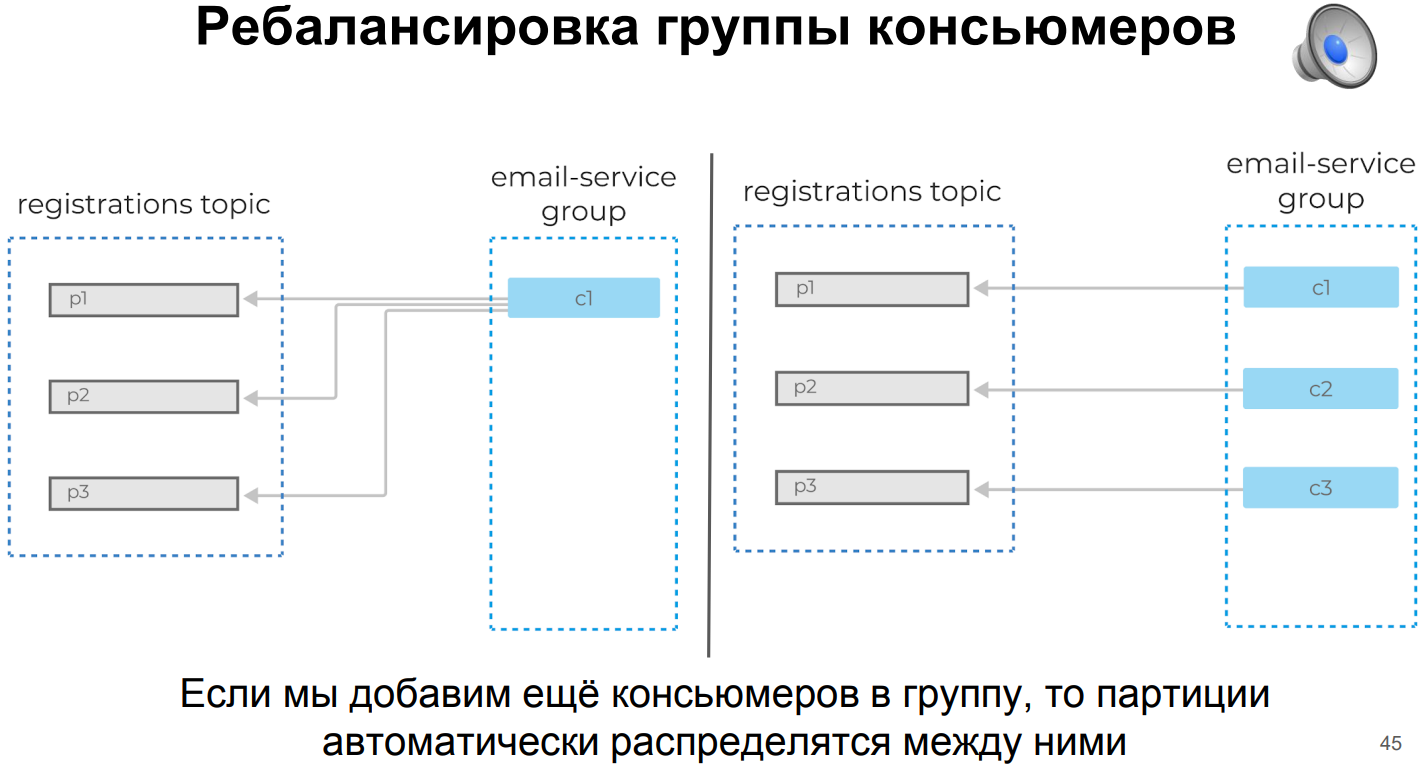
\includegraphics[width=\textwidth]{images/cgreb.png}
	\end{minipage}
\end{figure}

\begin{itemize}
    \item[+] Высокая пропускная способность, низкие задержки
    \item[+] Надежное отказоустойчивое хранение и эффективное масштабирование
    \item[+] Гибкие возможности по обеспечению разных семантик доставки данных
    \item[-] Нельзя ничего удалять (только по TTL)
    \item[-] Нельзя фильтровать сообщения не читая его
    \item[-] Слишком много партиций ведут к проблемам с открытыми файлами
    \item[-] Сложность входа
\end{itemize}


\subsection*{Kafka Stream, ksql, Spark Streaming.}

\textbf{Kafka streams} – фреймворк для обработки потоковых данных (не 
является составной частью Apache Kafka).

\textbf{KSQL и KSQLDb} - надстройка над Kafka Streams, позволяющая работать 
с потоками данных с помощью SQL-подобного языка.

\textbf{Spark Streaming и Spark Structured Streaming} - альтернатива 
приведенным выше технологиям.